\section{Introduction}
\subsection{Background and Organizational Structure of Host Organization}
\noindent
I am doing my ATAP at Government Technology Agency (GovTech), one of Singapore's statutory board. It is under the Prime Minister's Office (PMO) as shown in Figure \ref{fig:govtech-role}. It was restructured from the former entities Infocomm Development Authority of Singapore (IDA) and Media Development Authority (MDA) in 2016, and officially legislated in Parliament on 18 August 2016.\cite{REF1:1}
\begin{figure}[h!]
	\begin{center}
		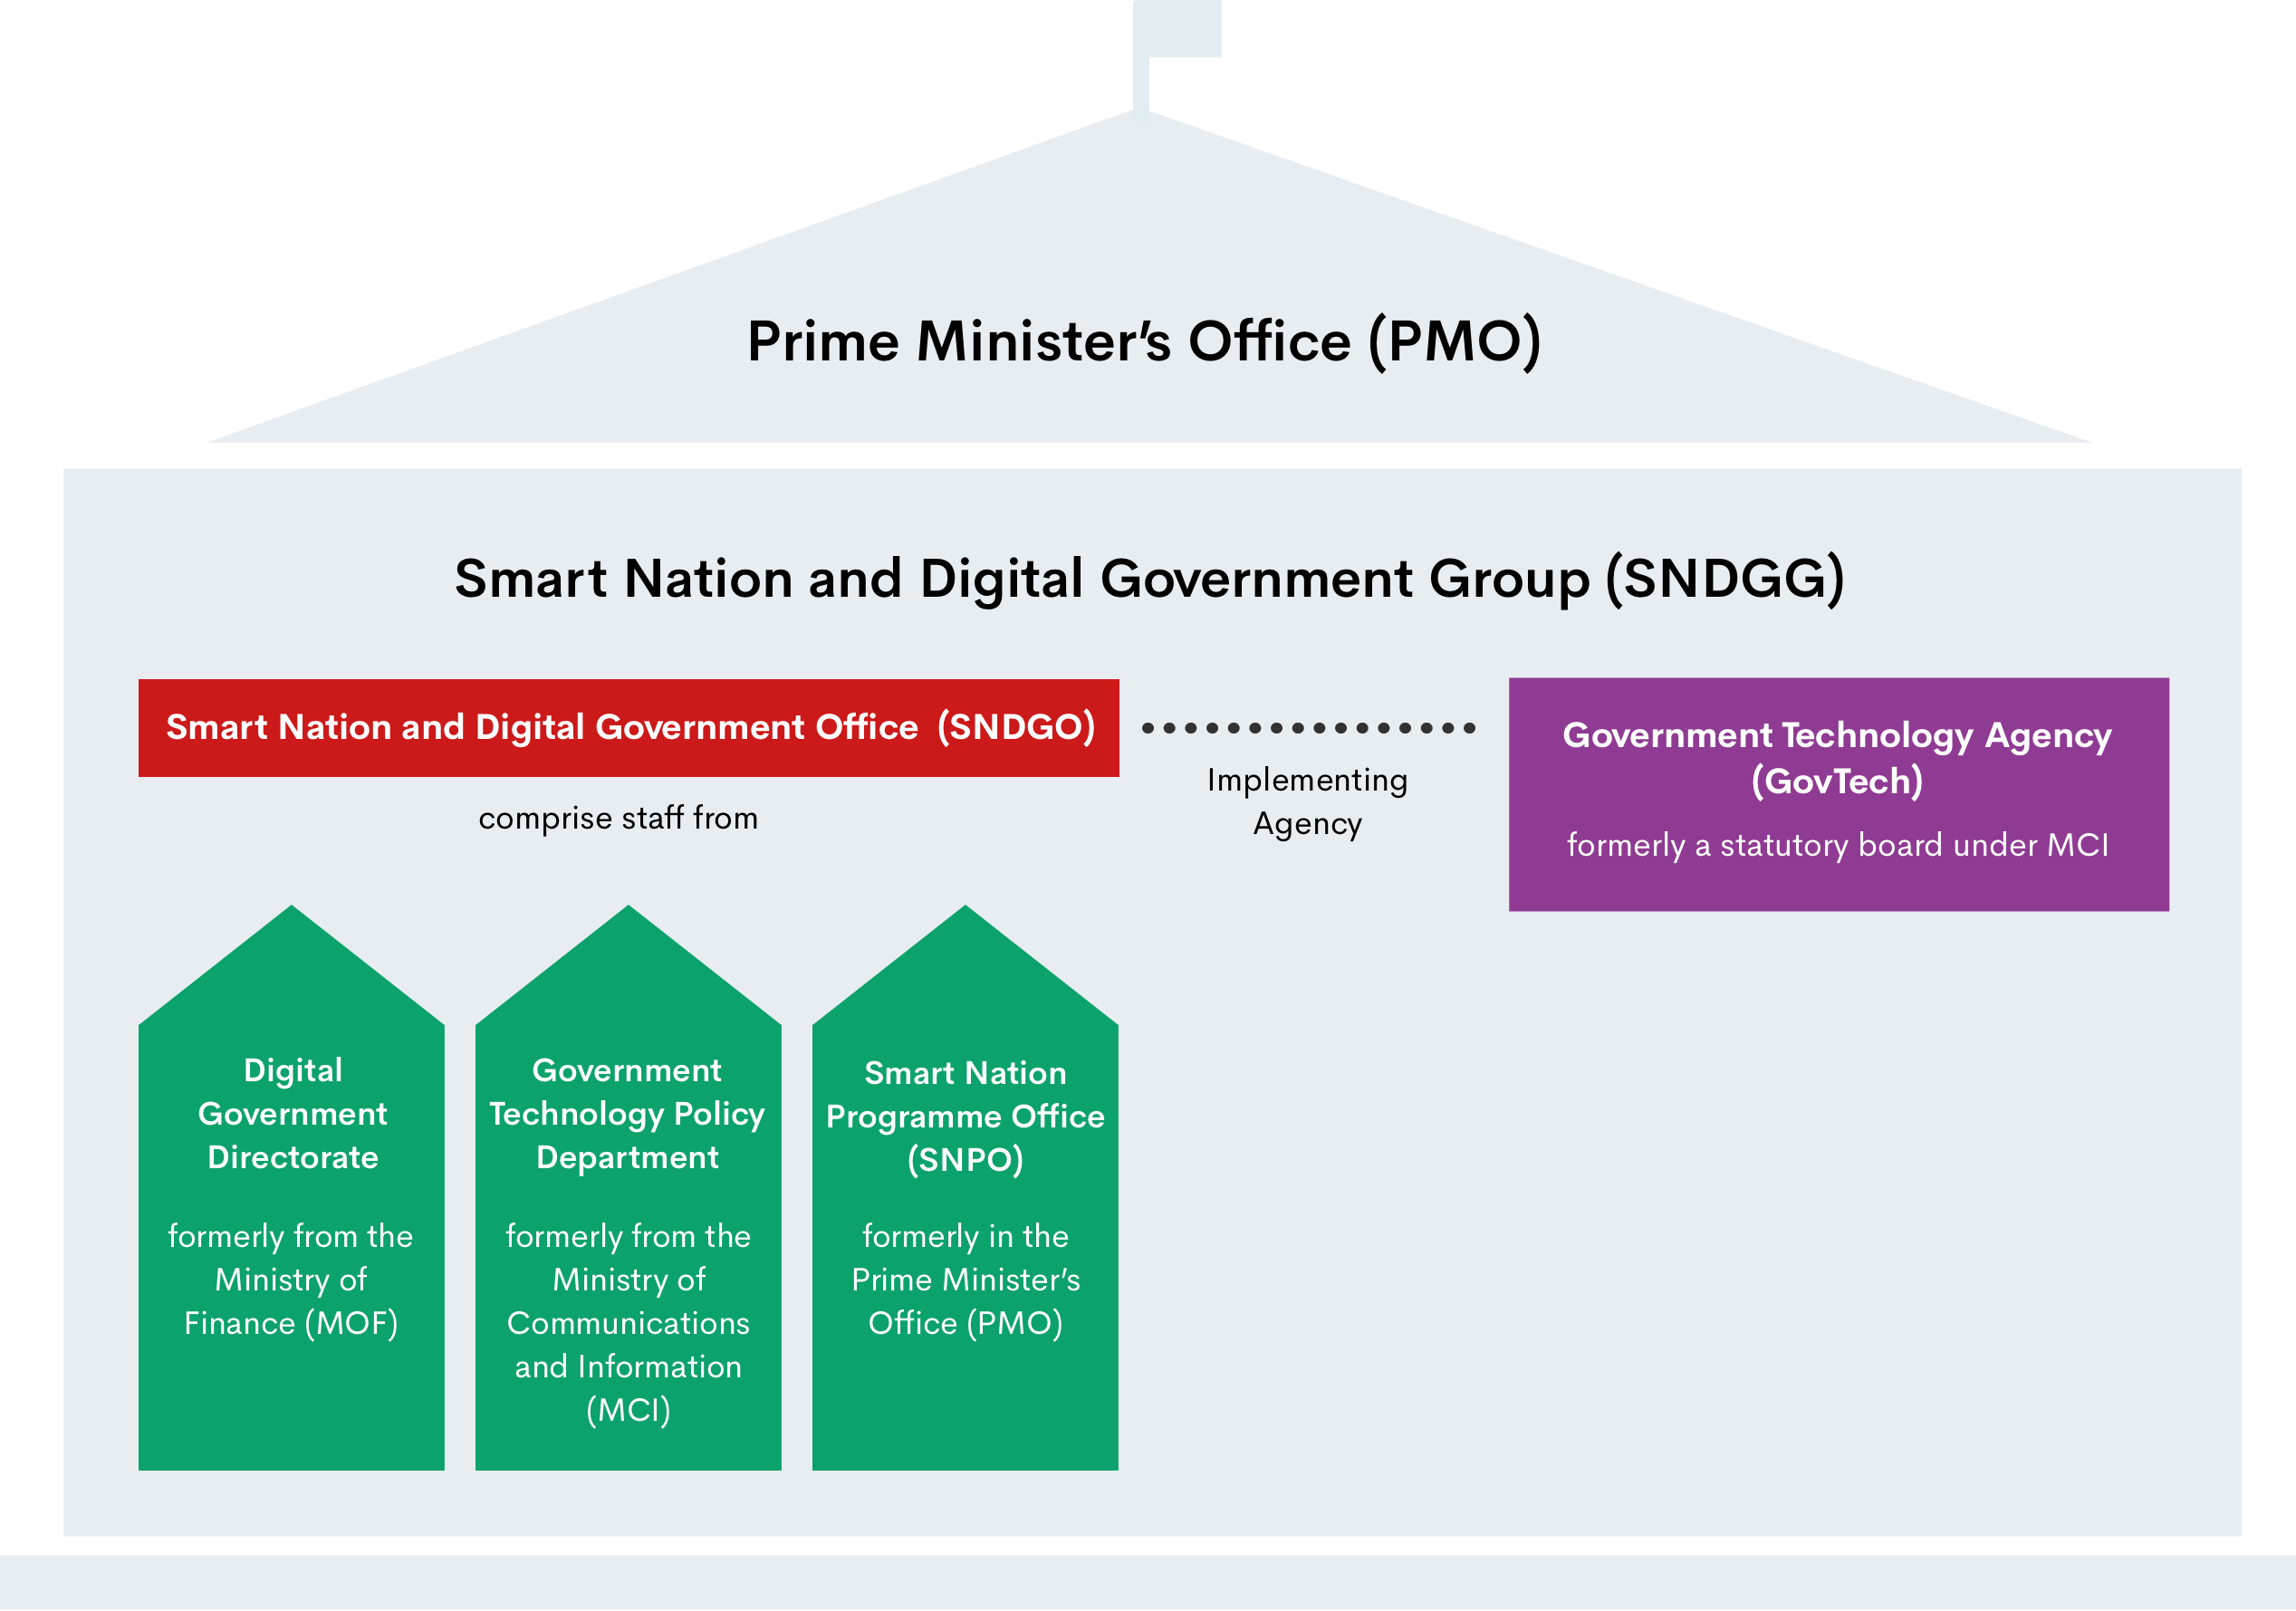
\includegraphics[width=300px]{assets/images/govtech-role.png}
		\caption{Organisational Chat For Smart Nation and Digital Governmnt Group (SNDGG) In Prime Minister Office\cite{REF2:1}}
		\label{fig:govtech-role}
	\end{center}
\end{figure}

\noindent
GovTech is created to spearhead Singapore's Smart Nation Initiatives and build capabilities in new technologies to shape the way business is done in the government. It focused on areas of Application Development, Cybersecurity, Data Science, Government ICT Infrastructure, and Sensors \& IoT.\cite{REF2:1}


\subsection{Principal Activities of Host Organization}
\noindent
GovTech outlined Singapore's Digital Government Blueprint (DGB) which is a statement of the Government's ambition to better leverage data and harness new technologies, and to drive broader efforts to build a digital economy and digital society as part of Singapore's Smart Nation Initiative. Its vision is to create a Government that is "Digital to the Core, and Serves with Heart". This means building user-centric services that cater to citizen's and businesses' needs. Using digital government services will also be easy and secure. Public officers will have opportunities to continually up-skill and adapt to new challenges.\cite{REF3:1}

\noindent
DGB will benefit the public by providing services that have digital signature options, are intuitive, are secured, and are catered for end users' needs. Examples of digital services that are already available and benefiting the public are Moments of Life, Business Grants Portal, and ParkingSG applications.\cite{REF3:1}

\subsection{Training Programme within Host Organization}
\noindent
GovTech has a leadership-trainee programme TAP which is designed to sharpen and develop technical knowledge and professional skills for fresh graduates. Participants will gain two years of specialist training and be groomed to take on specialist and technology leadership roles within GovTech that can also accelerate their career development.\cite{REF4:1}

\noindent
GovTech has developed a mobile application Learn GovSG where Public Officers can upgrade their skills through online videos. Teams in Govtech also organized workshops occasionally where others can signup and upgrade skills.\cite{REF5:1}

\subsection{Position of Host Unit within Host Organization}
\noindent
I am in the division Moments of Life (MOL). It is one of the Strategic National Projects under Singapore's Smart Nation Initiative that places citizens at the heart of digital government services at key life moments. It is a suite of services, which supports citizens' needs at key junctures by integrating and bundling services across Government agencies. It currently supports families with children aged 6 and below, and seniors aged 60 and above, by bundling useful services and information on a single digital platform.\cite{REF6:1}
